%-------------------------------------------------------------------------------
%-------------------------------------------------------------------------------
%-------------------------------------------------------------------------------
\chapter{Euler vectoriel}
%-------------------------------------------------------------------------------
%-------------------------------------------------------------------------------
\thispagestyle{empty}


Dans ce T.P. nous allons utiliser les tableaux \type{numpy} comme des vecteurs, nous allons tracer des représentations graphiques de solutions ou de portraits de phase et nous pourrons utiliser la méthode de résolution \type{odeint}.
%-------------------------------------------------------------------------------
\begin{lstlisting}
import numpy as np
import matplotlib.pyplot as plt
from scipy.integrate import odeint
\end{lstlisting}
%-------------------------------------------------------------------------------
%-------------------------------------------------------------------------------
%-------------------------------------------------------------------------------
\section{Systèmes différentiels}
%-------------------------------------------------------------------------------
%-------------------------------------------------------------------------------
%-------------------------------------------------------------------------------
Un système différentiel
$\displaystyle \left\{\begin{matrix}
x' = \phi_1(x, y, \ldots, t)\\
y' = \phi_2(x, y, \ldots, t)\\
\cdots
\end{matrix}\right.$
est considéré comme une équation différentielle d'ordre 1 dont la fonction à rechercher est une fonction à valeurs vectorielles. On écrit la fonction définissant l'équation différentielle sous la forme
\begin{lstlisting}
def phi(u, t):
    x, y, ... = u
    dx = # calcul de phi1(x, y, ..., t)
    dy = # calcul de phi2(x, y, ..., t)
    ...
    return np.array([dx, dy, ...])
\end{lstlisting}

La condition initiale sera aussi un tableau \type{numpy}
\begin{lstlisting}
u0 = np.array([x0, y0, ...])
\end{lstlisting}
La liste des temps peut être calculée par la fonction \type{numpy}
\begin{lstlisting}
T = np.linspace(t0, tFin, N)
\end{lstlisting}
On peut alors invoquer toutes les méthodes vues, le plus souvent \type{Euler} ou \type{odeint}
\begin{lstlisting}
U = Euler(phi, u0, T)
\end{lstlisting}
\type{U} est alors une liste de vecteurs dont on peut extraire les composantes
\begin{lstlisting}
X = [u[0] for u in U]
Y = [u[1] for u in U]
...
\end{lstlisting}
%-------------------------------------------------------------------------------
%-------------------------------------------------------------------------------
\subsection{Proies-prédateurs}
%-------------------------------------------------------------------------------
%-------------------------------------------------------------------------------
Un modèle d'évolution de deux espèces a été proposé dans les années 1920 par Alfred Lotka (1880-1949) et Vito Volterra (1860-1940). Il modélise les évolutions de deux type d'animaux, les {\bf proies}  et les {\bf prédateurs} dont les population sont représentées respectivement par les variables $p$ et $q$ {\bf à valeurs réelles}.

\begin{itemize}
  \item Les proies disposent de nourriture en quantité suffisante, en l'absence de prédateurs l'évolution est régie par un taux de natalité $\alpha$ : $\displaystyle \frac{\d p}{\d t} = \alpha p$. 
  \item Les prédateurs n'ont pas d'autre nourriture que les proies, en l'absence de celles-ci elles meurent avec un taux $\beta$ : $\displaystyle \frac{\d q}{\d t} = - \beta q$.
\item Les prédateurs peuvent croître (et les proies décroître) lors des rencontres dont le nombre est estimé proportionnel au produit $pq$ des populations. 
\end{itemize}
\[
\text{On parvient donc aux lois d'évolution}
\left\{
\begin{matrix}
\displaystyle \frac{\d p}{\d t} = \alpha p-\gamma pq\\
\\
\displaystyle \frac{\d q}{\d t} = -\beta q + \delta pq
\end{matrix} \right.\]

On donne les valeurs des coefficients dans des variables globales. Dans une étude théorique, on peut simplifier les valeurs.
\begin{lstlisting}
alpha = 1
beta  = 2
gamma = 0.001
delta = 0.001
\end{lstlisting}
%-------------------------------------------------------------------------------
%-------------------------------------------------------------------------------
\begin{Exercise}\it
Définir les fonctions de l'équation différentielle.

Résoudre cette équation sur $[0; 20]$ avec 10000 points pour les conditions initiales $p0= 6000$ et $q_0 = 1000$.

Tracer les solutions $p(t)$ et $q(t)$ en fonction de $t$ puis la trajectoire $\bigl(p(t), q(t)\bigr)$.
\end{Exercise}
%-------------------------------------------------------------------------------
\begin{Answer}
\begin{lstlisting}
def phi(u, t):
    p, q = u
    vp = alpha*p - gamma*p*q
    vq = beta*q + delta*p*q
    return np.array([vp, vq])

T = np.linspace(0, 20, 10000)
p0 = 6000
q0 = 1000
u0 = np.array([p0, q0])
U = Euler(phi, u0, T)
P = [u[0] for u in U]
Q = [u[1] for u in U]
plt.subplot(1, 2, 1)
plt.plot(T, P)
plt.plot(T, Q)
plt.subplot(1, 2, 2)
plt.plot(P, Q)
plt.show()
\end{lstlisting}
\begin{center}
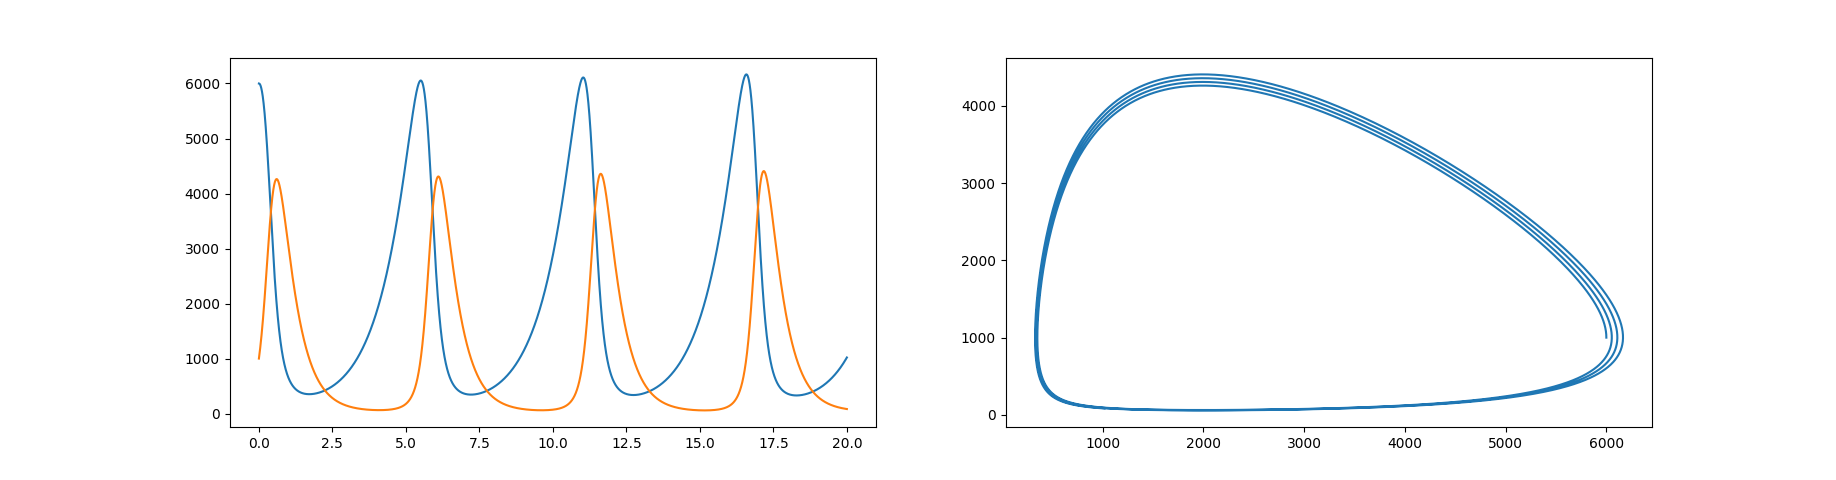
\includegraphics[width=14cm]{TP/Images/ED2_proies1.png}
\end{center}
\end{Answer}
%-------------------------------------------------------------------------------
%-------------------------------------------------------------------------------
On remarque que, si on a utilisé la méthode d'Euler, la trajectoire ne se referme pas. On peut prouver que les solutions décrivent une courbe fermée. Dans la suite on utilisera \type{odeint}.
%-------------------------------------------------------------------------------
%-------------------------------------------------------------------------------
\begin{Exercise}\it
Résoudre l'équation sur $[0; 20]$ avec 10000 points pour les conditions initiales $p0 \in \{2200, 2500, 3000, 4000, 6000, 10000\}$ et $q_0 = 1000$ et tracer, sur un même graphe les trajectoires.
\end{Exercise}
%-------------------------------------------------------------------------------
\begin{Answer}
\begin{lstlisting}
for p0 in [2200, 2500, 3000, 4000, 6000, 10000]:
    u0 = np.array([p0, q0])
    U = odeint(phi, u0, T)
    P = [u[0] for u in U]
    Q = [u[1] for u in U]
    plt.plot(P, Q)
plt.show()
\end{lstlisting}
\begin{center}
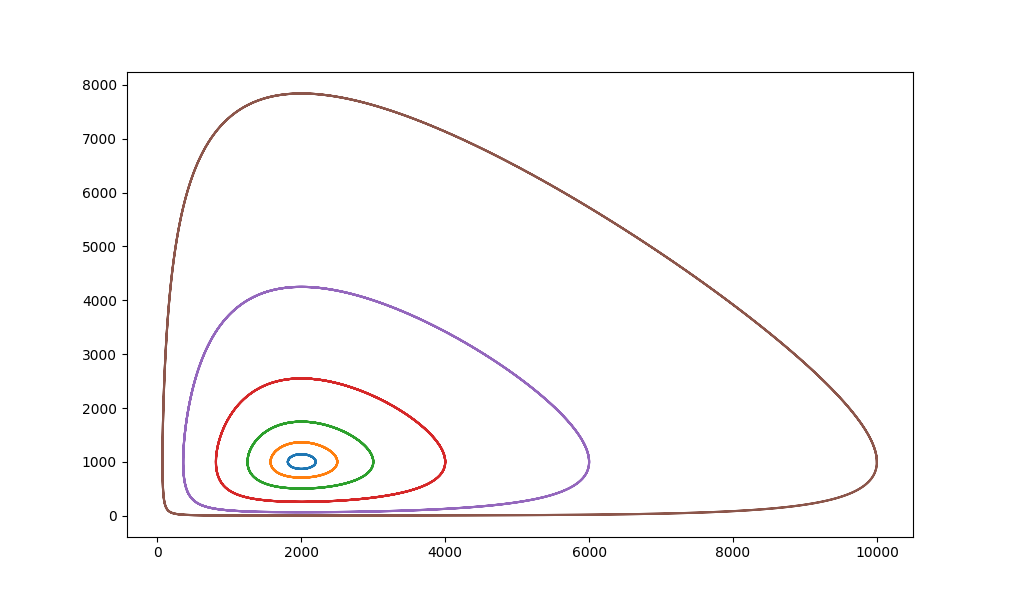
\includegraphics[width=12cm]{TP/Images/ED2_proies2.png}
\end{center}
\end{Answer}
%-------------------------------------------------------------------------------
%-------------------------------------------------------------------------------
\subsection{Simulation d'une épidémie}
%-------------------------------------------------------------------------------
%-------------------------------------------------------------------------------
On modélise la propagation d'une épidémie en séparant la population en 3 :
\begin{itemize}
    \item les individus {\bf sains} dont la proportion est représentée par une fonction $S(t)$,
    \item les personnes {\bf infectées} de proportion $I(t)$ et
    \item les guéris comptés par $R(t)$ (pour {\it recovered}).
\end{itemize}
On parle du modèle SIR.

On définit deux constantes $\beta$ et $\gamma$ qui représente respectivement le taux de transmission, c’est à dire le taux de personnes saines qui deviennent infectées par contact avec les personnes infectées et le taux de guérison, c’est à dire le taux de personnes infectées qui deviennent guéries. 

On suppose que les personnes guéries ne peuvent plus être infectées.

Mathématiquement, le modèle SIR est donné par le système :
\[\left\{
\begin{matrix}
\displaystyle \frac{\d S}{\d t}(t)&=&-\beta S(t)I(t)&&\\ 
\displaystyle \frac{\d I}{\d t}(t)&=&\beta S(t)I(t)&-&\gamma I(t)\\ 
\displaystyle \frac{\d R}{\d t}(t)&=&&&\gamma I(t)\\ 
\end{matrix}\right.\]

On note $R_0$ le rapport $\displaystyle \frac \beta\gamma$, il mesure la propagabilité de la maladie.

On prendra comme valeurs $R_0 = 3$ et $\gamma = 0.2$.

On considérera qu'on a $I(0) = 10^{-3}$ et $R(0) = 0$ et on étudiera l'évoilution pour $t\in [0;100]$

%--------------------------------------------------------------------------
%--------------------------------------------------------------------------
\begin{Exercise}\it 
Tracer, sur un même graphique, les proportions de chaque type de population pour $t$ variant entre 0 et 100.
\end{Exercise}
%--------------------------------------------------------------------------
\begin{Answer}
\begin{lstlisting}
R0 = 3
gamma = 0.2
beta = R0*gamma

def phi(u, t):
    s, i, r = u
    return np.array([-beta*s*i, beta*s*i - gamma*i, gamma*i])

i0 = 1e-3
CI = np.array([1-i0, i0, 0])
t_max = 100
T = np.linspace(0, t_max, 10000)
U = odeint(phi, CI, T)
plt.plot(T,U)
plt.show()
\end{lstlisting}
%--------------------------------------------------------------------------
\begin{center}
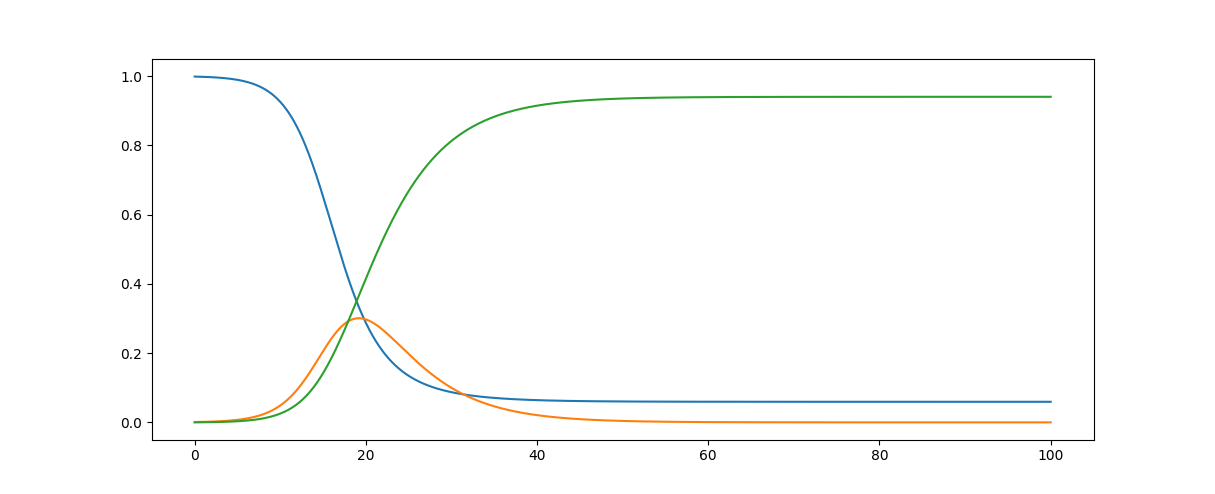
\includegraphics[width=12cm]{TP/Images/ED2_SIR1.png}
\end{center}
\newpage
\end{Answer}
%-------------------------------------------------------------------------------
%--------------------------------------------------------------------------
On ajoute une période de confinement entre les temps $t= 10$ et $t = 40$, pendant laquelle le coefficient $R0$ est divisé par 2, $\gamma$ restant constant.
%--------------------------------------------------------------------------
%--------------------------------------------------------------------------
\begin{Exercise}\it 
Après avoir défini une nouvelle fonction $\phi$, tracer, sur un même graphique, les proportions de chaque type de population.
\end{Exercise}
%--------------------------------------------------------------------------
\begin{Answer}
\begin{lstlisting}
def phi(u, t):
    if 10 < t < 40:
        bet = beta/2
    else:
        bet = beta
    s, i, r = u
    return np.array([-bet*s*i, bet*s*i - gamma*i, gamma*i])

i0 = 0.01
CI = np.array([1 - i0, i0, 0])
t_max = 100
T = np.linspace(0, t_max, 10000)
U = odeint(phi, CI, T)
plt.plot(T,U)
plt.show()
\end{lstlisting}
%--------------------------------------------------------------------------
\begin{center}
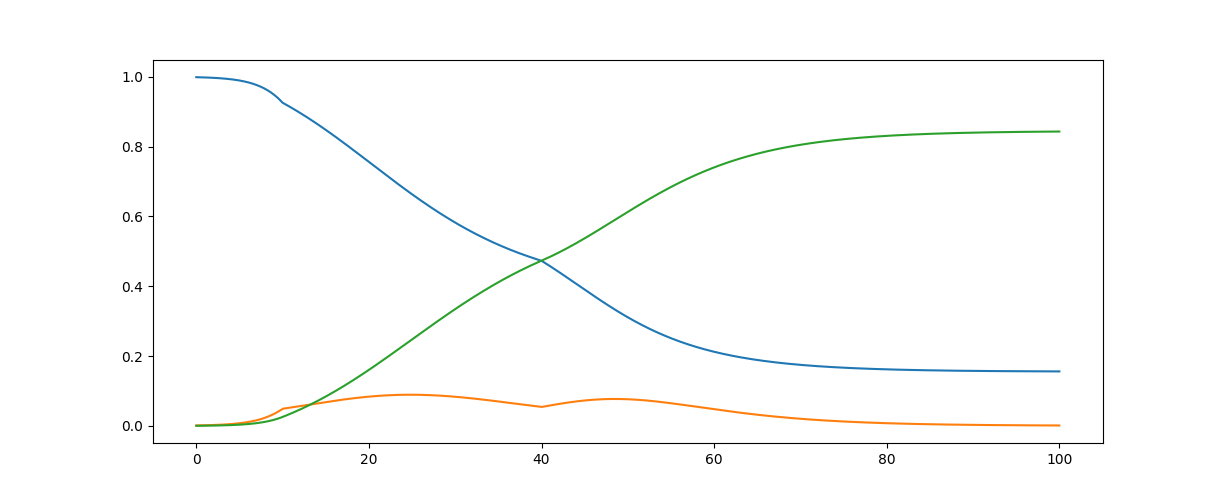
\includegraphics[width=12cm]{TP/Images/ED2_SIR2.png}
\end{center}
\end{Answer}
%-------------------------------------------------------------------------------
%-------------------------------------------------------------------------------
\subsection{Équations de Lorenz}
%-------------------------------------------------------------------------------
%-------------------------------------------------------------------------------
Lors de l'étude des phénomènes météorologiques, Edward Lorenz a simplifié, en 1963, les équations issues de la mécanique des fluides en un système dynamique tridimensionnel. Ce système engendre un comportement chaotique dans certaines conditions. Il est donné par
\[\left\{\begin{matrix}
x'&=&\sigma(y-x)\\ 
y' &=& \rho x - y - xz\\
z'&=& xy - \beta z\\
\end{matrix}\right.\]
avec $\sigma = 10$, $\rho = 28$ et $\beta = 8/3$.
On peut tracer une trajectoire dans l'espace avec la fonction \type{Axes3D}.
\begin{lstlisting}
from mpl_toolkits.mplot3d import Axes3D
\end{lstlisting}

Le tracé 3D est fait en définissant un cadre ; \type{mon\_dessin} est le nom choisi.

Pour les version de \type{numpy} jusqu'à 3.3
\begin{lstlisting}
fig = plt.figure()
mon_dessin = Axes3D(fig)
\end{lstlisting}

Pour les version de \type{numpy} à partir de 3.4
\begin{lstlisting}
fig = plt.figure()
mon_dessin = Axes3D(fig, auto_add_to_figure = False)
fig.add_axes(mon_dessin)
\end{lstlisting}

On peut alors tracer la trajectoire, définie par 3 listes \type{X}, \type{Y} et \type{Z} de même longueur.
\begin{lstlisting}
mon_dessin.plot(X, Y, Z) 
plt.show()
\end{lstlisting}
%-------------------------------------------------------------------------------
%-------------------------------------------------------------------------------
\begin{Exercise}\it
Tracer le portrait de phase sur $[0;30]$ pour les conditions initiales $x(0) =0.1$, $y(0) =0$ et $z(0) =0.1$.
\end{Exercise}
%--------------------------------------------------------------------------
\begin{Answer}
\begin{lstlisting}
def lorenz(u, t):
    sigma = 10
    rho = 28
    beta = 8/3
    x, y, z = u
    vx = sigma*(y - x)
    vy = rho*x - y - x*z
    vz = x*y - beta*z
    return np.array([vx, vy, vz])

T = np.linspace(0, 30, 10000)
y0 = np.array([0.1, 0.0, 0.1])
U = odeint(lorenz, y0, T)
X = [u[0] for u in U]
Y = [u[1] for u in U]
Z = [u[2] for u in U]

fig = plt.figure()
mon_dessin = Axes3D(fig, auto_add_to_figure = False)
fig.add_axes(mon_dessin)

mon_dessin.plot(X, Y, Z) 
plt.show()
\end{lstlisting}
%--------------------------------------------------------------------------
\begin{center}
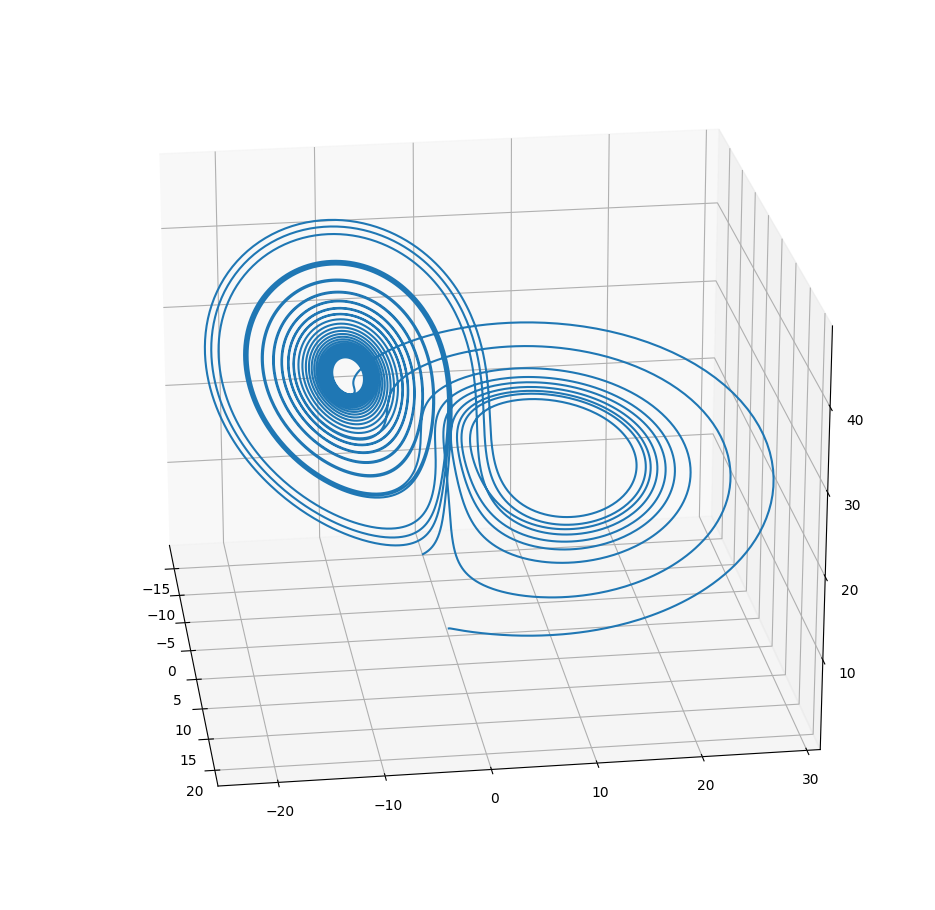
\includegraphics[width=10cm]{TP/Images/ED2_Lorenz.png}
\end{center}
%-------------------------------------------------------------------------------
\end{Answer}
%-------------------------------------------------------------------------------
%-------------------------------------------------------------------------------
\newpage
%-------------------------------------------------------------------------------
\section{Équations d'ordre 2}
%-------------------------------------------------------------------------------
%-------------------------------------------------------------------------------
%-------------------------------------------------------------------------------
On rappelle que, pour résoudre ces équations, on introduit une variable supplémentaire, la dérivée de $y$, notée ici $v$. L'équation $y''= \psi(y, y', t)$ devient alors le système 
\[\left\{
\begin{matrix}
  y' = v\\
  v' = \psi(y, v, t)
\end{matrix}
\right.\]
%-------------------------------------------------------------------------------
%-------------------------------------------------------------------------------
\subsection{Un exemple simple avec erreur d'arrondi}
%--------------------------------------------------------------------------
%--------------------------------------------------------------------------
\begin{Exercise}[label={exo:EDL2cc}]
\it Tracer les solutions de 
$y'' = 2y$ avec $y(0)=1$ et $y'(0) = -\sqrt 2$ sur $[0;30]$.
\end{Exercise}
%--------------------------------------------------------------------------
\begin{Answer}
La solution générale est $A.e^{\sqrt 2t} + B.e^{-\sqrt 2 t}$. Les conditions initiales imposent $y(t) = e^{-\sqrt 2t}$ mais les erreurs d'arrondi et d'imprécision font que la solution calculée comporte un terme en $e^{\sqrt 2t}$ avec un coefficient très petit mais dont le produit par $e^{2t}$ finit par ne plus être négligeable.
\begin{lstlisting}
def phi(u, t):
    y, v = u
    a = 2*y
    return np.array([v, a])

T = np.linspace(0, 30, 10000)
u0 = np.array([1, -2**0.5])
U = odeint(phi, u0, T)
Y = [u[0] for u in U]
plt.plot(T, Y)
plt.ylim([-10, 2])
plt.show()
\end{lstlisting}
%--------------------------------------------------------------------------
\begin{center}
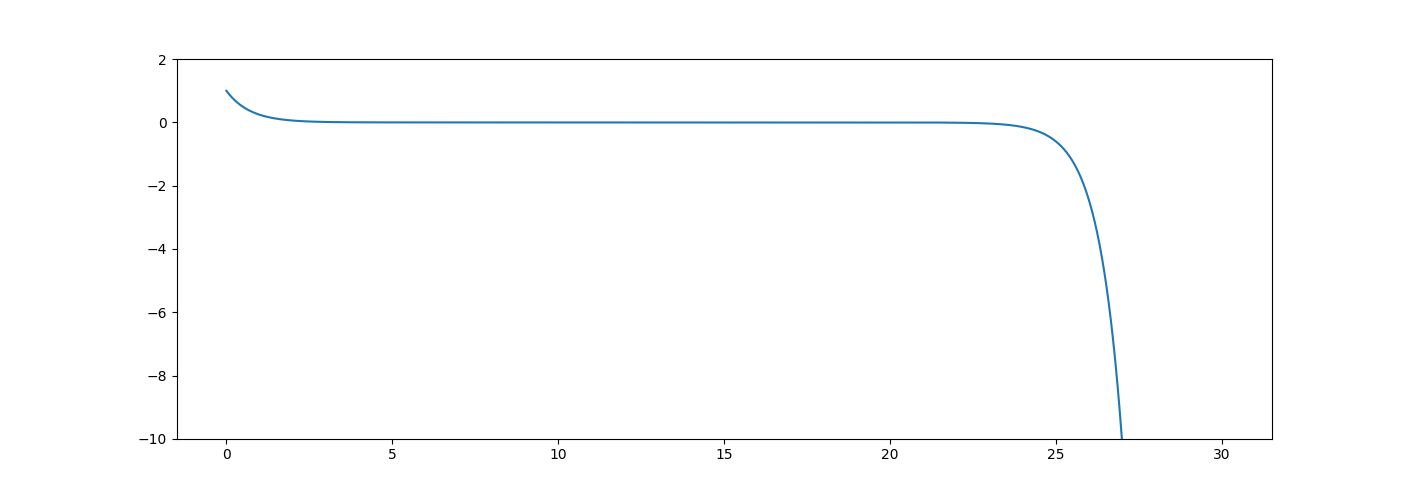
\includegraphics[width=13cm]{TP/Images/ED2_erreur.png}
\end{center}
%-------------------------------------------------------------------------------
\end{Answer}
%--------------------------------------------------------------------------
%-------------------------------------------------------------------------------
\subsection{Pendule asymétrique}
%--------------------------------------------------------------------------
%--------------------------------------------------------------------------
\begin{minipage}[c]{.60\linewidth}
Une masse $m$ est fixée sur une tige rigide de longueur $l$, solidaire d'une poulie de rayon $R$. Un fil est enroulé autour de la poulie, une masse $M$ étant fixée à son extrémité libre.

Le fil étant inextensible, $z=R\theta$. Le problème est ainsi ramené à un système à un seul degré de liberté $\theta$. 
Son énergie mécanique $E_m$ est une constante qui s'exprime à tout instant par :
	\[
	E_m=\frac{1}{2}(ml^2+MR^2)\dot{\theta}(t)^2+mgl(1-\cos\bigl(\theta(t))\bigr)-MgR\theta
	\]
que l'on ramène par dérivation à :
	\[
	\ddot{\theta}(t)+\frac{mgl\sin\bigl(\theta(t)\bigr)-MgR}{ml^2+MR^2}=0
	\]
\end{minipage}  
%--------------------------------------------------------------------------
\begin{minipage}[c]{.40\linewidth}
\begin{center}
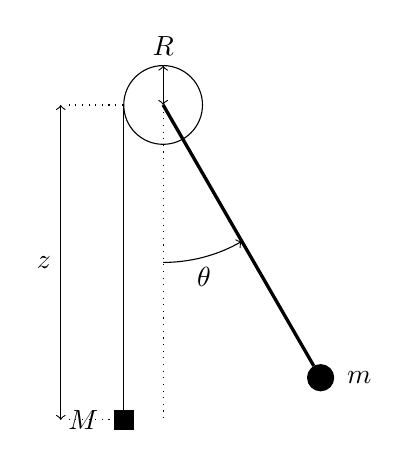
\begin{tikzpicture}
\draw[dotted] (-1.2, 0) -- (-0.5, 0);
\draw[dotted] (-1.2, -4) -- (-0.5, -4);
\draw(0, 0) circle (0.5);
\draw[<->] (0, 0) -- (0, 0.5) node[above] {$R$};
\draw (-0.5, -4) node[rectangle, draw,fill] (M){}; 
\draw (-0.5, 0) -- (M) node[left=2mm]{$M$};
\draw (300:4) node[circle, draw,fill] (m){}; 
\draw[very thick] (0, 0) -- (m) node[right=2mm]{$m$};
\draw[dotted] (0, 0) -- (0, -4);
\draw[->] (0, -2) arc (270:300:2) node [midway, below] {$\theta$};
\draw[<->] (-1.3, 0) -- node [left] {$z$} +(0, -4);
\end{tikzpicture}  
\end{center}
\end{minipage}  
%--------------------------------------------------------------------------

\medskip


Si $M$ est trop lourde, $m$ ne pourra pas l'empêche de chuter. Alors la tige va entrer en révolution autour de la poulie : $\theta$ sera non bornée. Idem si l'une des deux masses se voit imprimer une vitesse initiale trop importante. Sinon, les deux masses oscilleront, l'une angulairement et l'autre linéairement, autour d'une position d'équilibre.
%--------------------------------------------------------------------------
\begin{lstlisting}
R = 0.05  #m
l = 0.5   #m
m = 0.1   #kg
g = 9.81  #m.s^{-2}
\end{lstlisting}
--------------------------------------------------------------------------

%--------------------------------------------------------------------------
%--------------------------------------------------------------------------
\begin{Exercise}\it 
Tracer les solutions pour le temps variant entre 0 et 5s, pour $M$ prenant les valeurs :  0,65kg, 0,70 kg, 0.72 kg, 0.73 kg  et pour les conditions initiales : $\theta(0)=0$ et $\dot{\theta}(0)=0$.
\end{Exercise}
%--------------------------------------------------------------------------
\begin{Answer}
\begin{lstlisting}
def phi(u, t):
    y, v = u
    a = (M*g*R - m*g*l*np.sin(y)) / (m*l**2 + M*R**2)
    return np.array([v, a])

N = 10000
tmin = 0
tmax = 5

CI = np.array([0, 0])
T = np.linspace(tmin, tmax, N)
liste_M = [0.65, 0.70, 0.72, 0.73]
for M in liste_M:
    U = odeint(phi, CI, T)
    Y = [u[0] for u in U]
    plt.plot(T, Y, label = "Position pour M={}".format(M))

plt.legend()
plt.show()
\end{lstlisting}
%--------------------------------------------------------------------------
\begin{center}
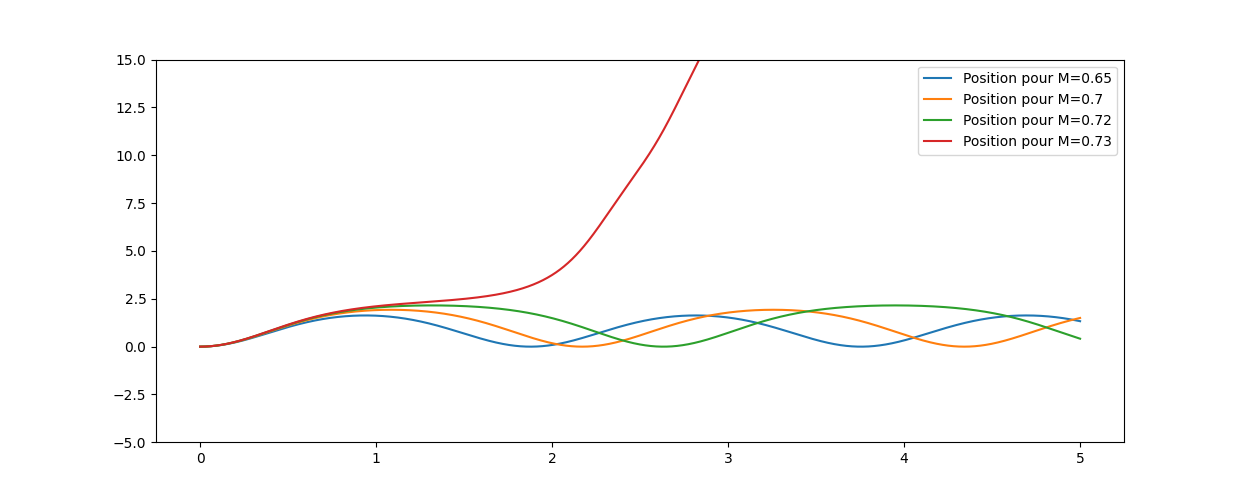
\includegraphics[width=16cm]{TP/Images/ED2_asym1.png}
\end{center}
%--------------------------------------------------------------------------
\end{Answer}
%--------------------------------------------------------------------------
%--------------------------------------------------------------------------
\begin{Exercise}\it 
Tracer, sur un même graphique, les portraits de phases on se restreindra à l'intervalle $[0; 2,5]$ pour le temps
\end{Exercise}
%--------------------------------------------------------------------------
\begin{Answer}
\begin{lstlisting}
tmax = 2.5
CI = np.array([0, 0])
T = np.linspace(tmin, tmax, N)
liste_M = [0.65, 0.72, 0.74]
liste_M = [0.65, 0.70, 0.72, 0.73]
for M in liste_M:
    U = odeint(phi, CI, T)
    Y = [u[0] for u in U]
    V = [u[1] for u in U]
    plt.plot(Y, V, label = "Position pour M={}".format(M))

plt.legend()
plt.show()
\end{lstlisting}
%--------------------------------------------------------------------------
\begin{center}
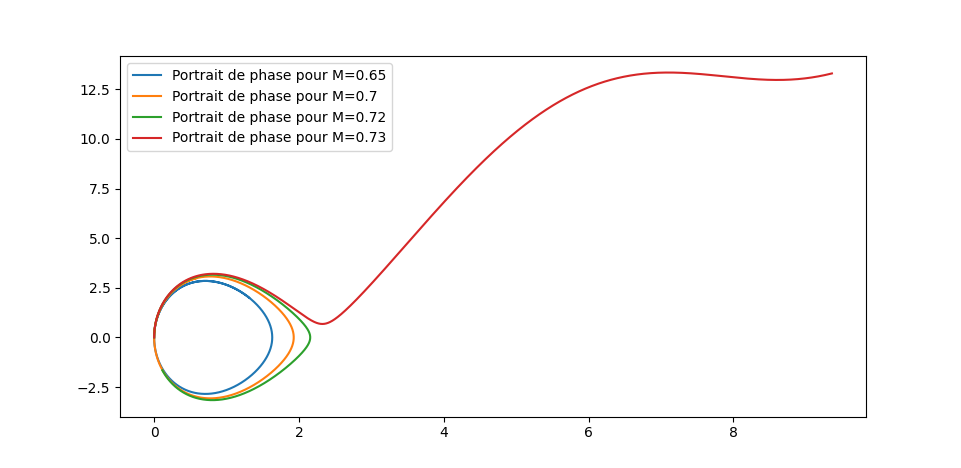
\includegraphics[width=16cm]{TP/Images/ED2_asym2.png}
\end{center}
\end{Answer}
%-------------------------------------------------------------------------------
\newpage
%-------------------------------------------------------------------------------
\subsection{Équation de van der Pol}
%-------------------------------------------------------------------------------
%-------------------------------------------------------------------------------
Ce qui suit est tiré de Wikipedia

\begin{minipage}{.45\linewidth}
L’oscillateur de Van der Pol a été imaginé par le physicien néerlandais Balthasar van der Pol alors qu'il était employé par les laboratoires {\sc Philips}. Van der Pol découvrit que le circuit ci-contre contenant un tube à vide développait des oscillations stables, qu'il appela \emph{oscillation de relaxation} et que l'on désigne aujourd'hui plutôt comme des cycles limites des circuits électriques.

L'équation vérifiée par  $u_g$ est
\[y'' = \varepsilon\omega_0(1-y^2)y'-\omega_0^2y\]
\end{minipage}
%--------------------------------------------------------------------------
\begin{minipage}[c]{.55\linewidth}
  \begin{center}
    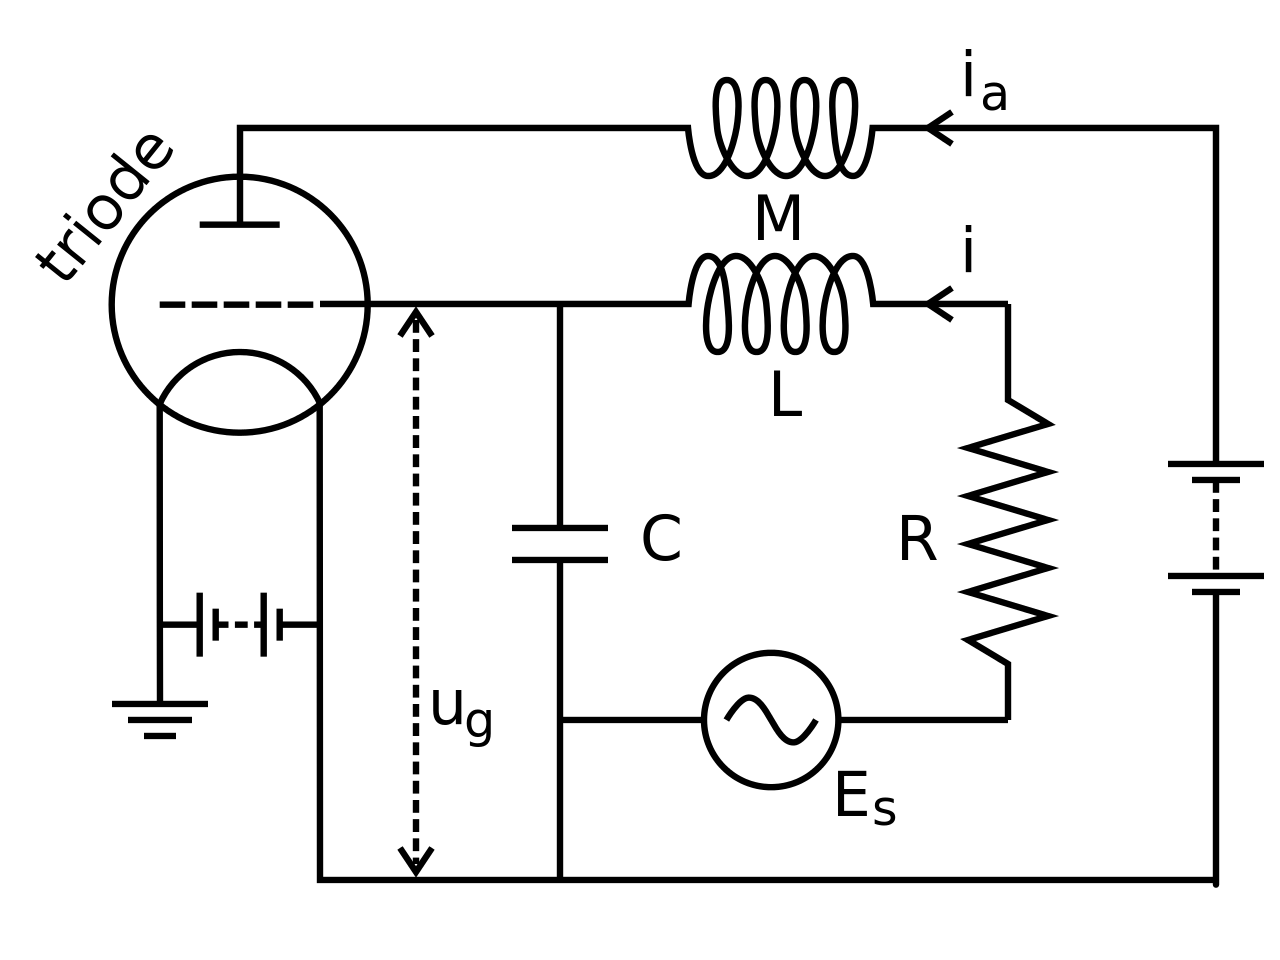
\includegraphics[width=7cm]{TP/Images/ED2_van_der_pol.png}
   \end{center}
\end{minipage}
%-------------------------------------------------------------------------------
\medskip

Dans la suite on prendra $\varepsilon = \omega_0=1$.
\textbf{}\begin{lstlisting}
epsilon = 1
omega0 = 1
\end{lstlisting}
%-------------------------------------------------------------------------------
%-------------------------------------------------------------------------------
\begin{Exercise}\it
Écrire la fonction \type{phi(y, v, t)} correspondant à l'équation.

Tracer le portrait de phase de la solution sur $[0;20]$ pour différentes conditions initiales : 
$y_0 \in \{1, 3, 5\}$ et $ v_0 \in \{-3, 0, 3\}$. 
\end{Exercise}
%-------------------------------------------------------------------------------
\begin{Answer}
\begin{lstlisting}
def phi(u, t):
    y, v = u
    a = epsilon*omega0*(1-y**2)*v -omega0**2*y
    return np.array([v, a])

T = np.linspace(0, 20, 10000)
for y0 in [1, 3, 5]:
    for v0 in [-3, 0, 3]:
        u0 = np.array([y0, v0])
        U = odeint(phi, np.array(u0), T)
        Y = [u[0] for u in U]
        V = [u[1] for u in U]
        plt.plot(Y, V)
plt.show()
\end{lstlisting}
%--------------------------------------------------------------------------
\begin{center}
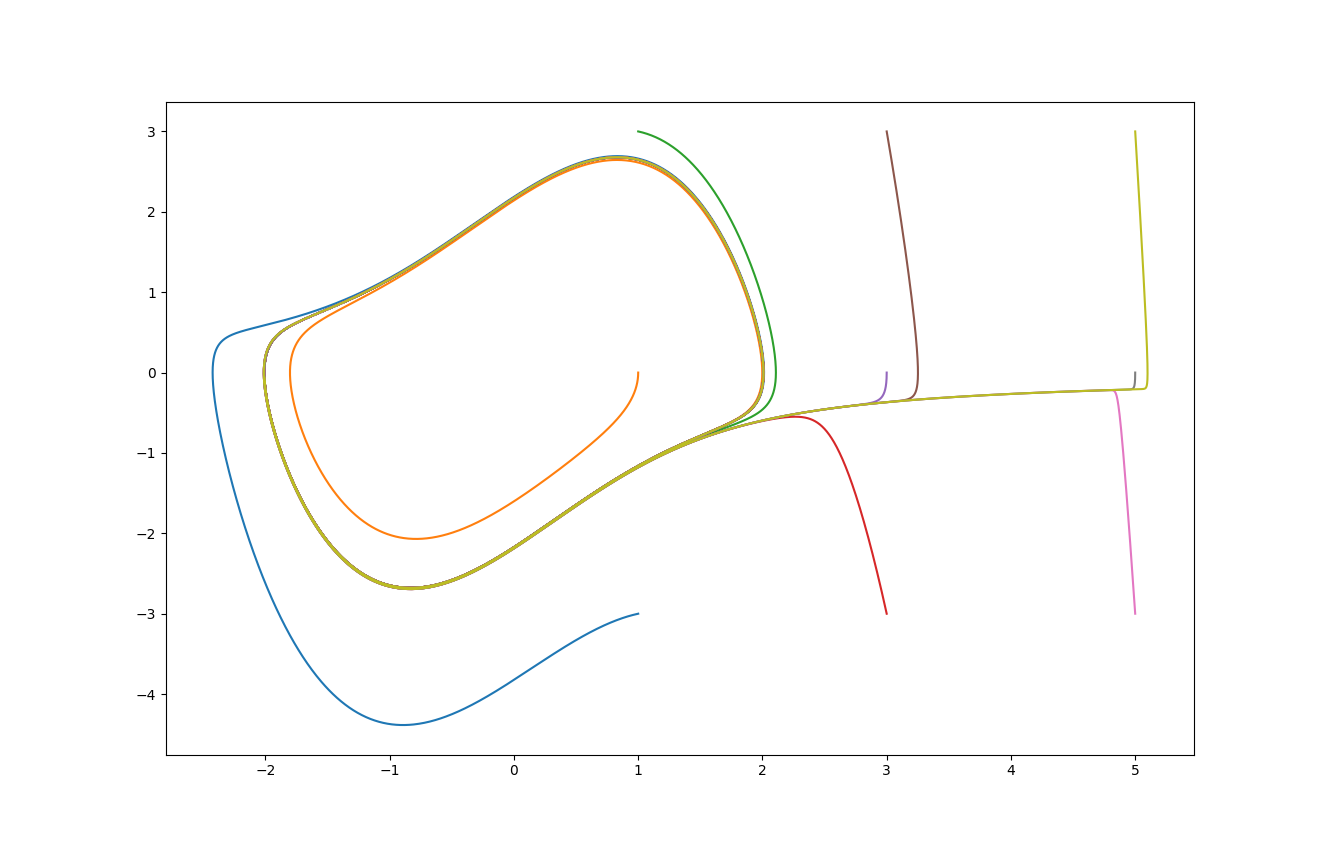
\includegraphics[width=12cm]{TP/Images/ED2_vdp_cycle.png}
\end{center}
%-------------------------------------------------------------------------------
\end{Answer}
%-------------------------------------------------------------------------------
%-------------------------------------------------------------------------------
On remarque que les courbes finissent par se ressembler, c'est le cycle limite.
%-------------------------------------------------------------------------------
%-------------------------------------------------------------------------------
%-------------------------------------------------------------------------------
\section{Systèmes différentiels d'ordre 2}
%-------------------------------------------------------------------------------
%-------------------------------------------------------------------------------
%-------------------------------------------------------------------------------
On peut généraliser et étudier des sustèmes de polusieurs équations différentielles couplées d'ordre 2. On se ramène à un système d'ordre 1 en dédoublant les variables : à chaque variable on lui associe sa dérivée.
%--------------------------------------------------------------------------
%-------------------------------------------------------------------------------
\subsection{Effet Zeeman}
%-------------------------------------------------------------------------------
%-------------------------------------------------------------------------------
L'électron dans l'atome est classiquement modélisé comme «élastiquement lié» : un point matériel de masse $m$ et de charge électrique $e$, repéré par sa position $\vec{r}$, et soumis de la part du noyau à une force de rappel élastique, anticolinéaire à $\vec{r}$. Il se comporte alors comme un oscillateur harmonique de pulsation $\omega_0$.

Si l'atome est soumis à un champ magnétique $\vec{B}$ colinéaire à $\vec{u}_z$, il subit une seconde force, d'origine magnétique ; il se produit alors un phénomène appelé effet Zeeman :
	\begin{itemize}
	\item L'électron garde un mouvement oscillant à la pulsation $\omega_0$ le long du champ magnétique.
	\item Il développe un mouvement bi-harmonique dans le plan perpendiculaire au champ magnétique, aux pulsations $\omega_0\pm\Omega$, où $\Omega$ est une pulsation proportionnelle au champ magnétique.
	\item L'atome peut alors émettre un rayonnement sur les trois pulsations $\omega_0$, $\omega_0-\Omega$ et $\omega_0+\Omega$.
	\end{itemize}
Le mouvement suivant $z$ est un simple oscillateur harmonique découplé des deux autres, donc il ne sera pas étudié.

%-------------------------------------------------------------------------------
L'équation différentielle gouvernant le vecteur position est 
$\vec{r}\,''(t)+\frac em\vec{r}\,'(t)\wedge\vec{B}+\omega_0^2\vec{r}=\vec{0}$.
Elle se traduit en le système
$\left\{\begin{matrix}
\ddot{x}+\omega_0^2x &=& -2\omega\dot{y}\\ 
\ddot{y}+\omega_0^2y &=& 2\omega\dot{x}
\end{matrix}\right.$
avec $\omega=\frac{eB}{2m}$.

\newpage
L'équation différentielle portera donc sur 4 variables :
\begin{lstlisting}
def phi(u, t):
    x, y, vx, vy = u
    ax = ...
    ay = ...
    return np.array([vx, vy, ax, ay])
\end{lstlisting}


On choisit, pour conditions initiales, $\vec{r}(0)=\vec{0}$ 
et $\vec{r}\,'(0)=a\omega_0\vec{u}_x$.

Valeurs numériques :\footnote{La valeur numérique du champ magnétique est énormément amplifiée pour les besoins de cet exercice, sans ça le phénomène est difficile à voir sur un graphique.}
\begin{lstlisting}
m = 9.1e-31    #kg, masse de l'électron
e = 1.6e-19    #C, charge de l'électron
w0 = 4.34e15   #rad/s pulsation propre du rappel du noyau
B = 1000       #T, intensité du champ magnétique

w = (e*B)/(2*m)
a = 5.3e-11
\end{lstlisting}
%-------------------------------------------------------------------------------
%-------------------------------------------------------------------------------
\begin{Exercise}\it
Tracer le graphe des solutions $x(t)$ et $y(t)$ sur $[0; 5.10^{-14}]$.

Tracer le diagramme des phases pour la solution $x(t)$.
\end{Exercise}
%--------------------------------------------------------------------------
\begin{Answer}
\begin{lstlisting}
def zeeman(u, t):
    x, y, vx, vy = u
    ax = -2*w*vy-w0**2*x
    ay = 2*w*vx-w0**2*y
    return np.array([vx, vy, ax, ay])

t_max = 5e-14
T = np.linspace(0, t_max, 3000)

r0x = 0
r0y = 0
v0x = a*w0
v0y = 0
CI = np.array([r0x, r0y, v0x, v0y])


U = odeint(zeeman, CI, T)
X = [u[0] for u in U]
Y = [u[1] for u in U]
VX = [u[2] for u in U]
VY = [u[3] for u in U]

plt.plot(T, X, label = "$x(t)$")
plt.plot(T, Y, label = "$y(t)$")
plt.legend()
plt.show()
\end{lstlisting}
%--------------------------------------------------------------------------
\begin{center}
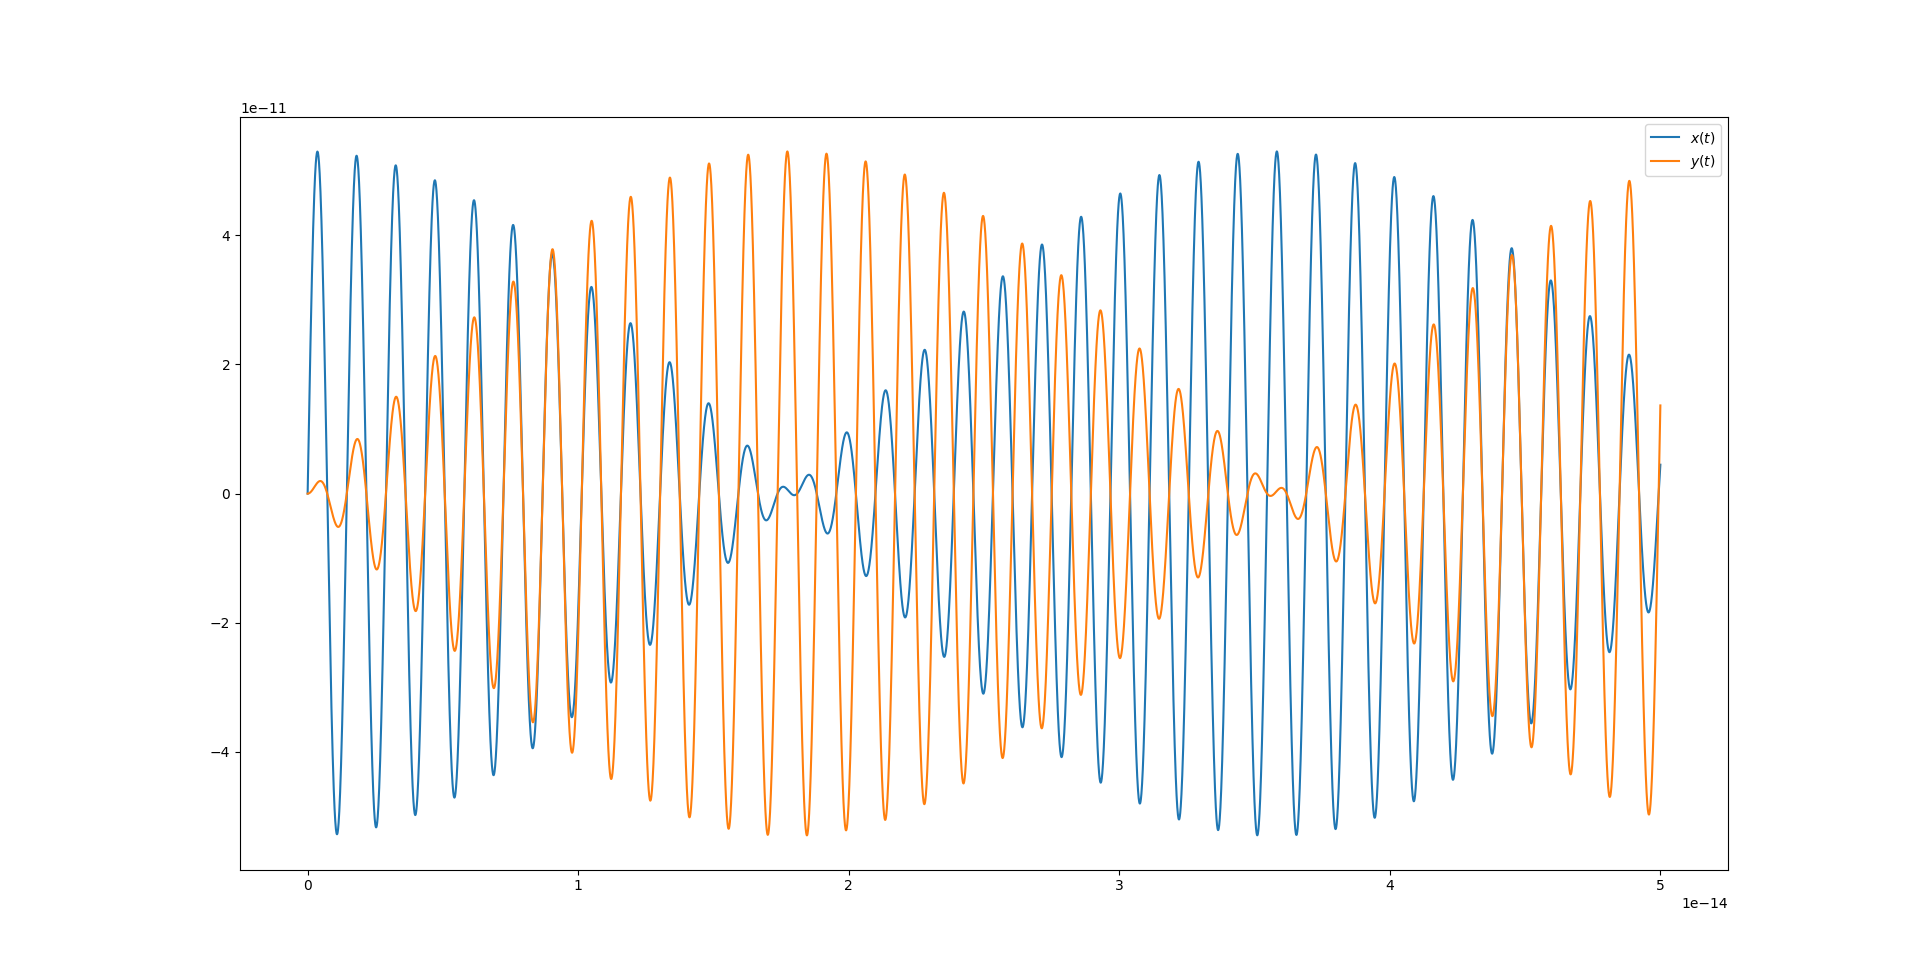
\includegraphics[width=12cm]{TP/Images/ED2_Zeeman1.png}    
\end{center}
%-------------------------------------------------------------------------------
\begin{lstlisting}
plt.plot(X, VX)
plt.show()
\end{lstlisting}
%--------------------------------------------------------------------------
\begin{center}
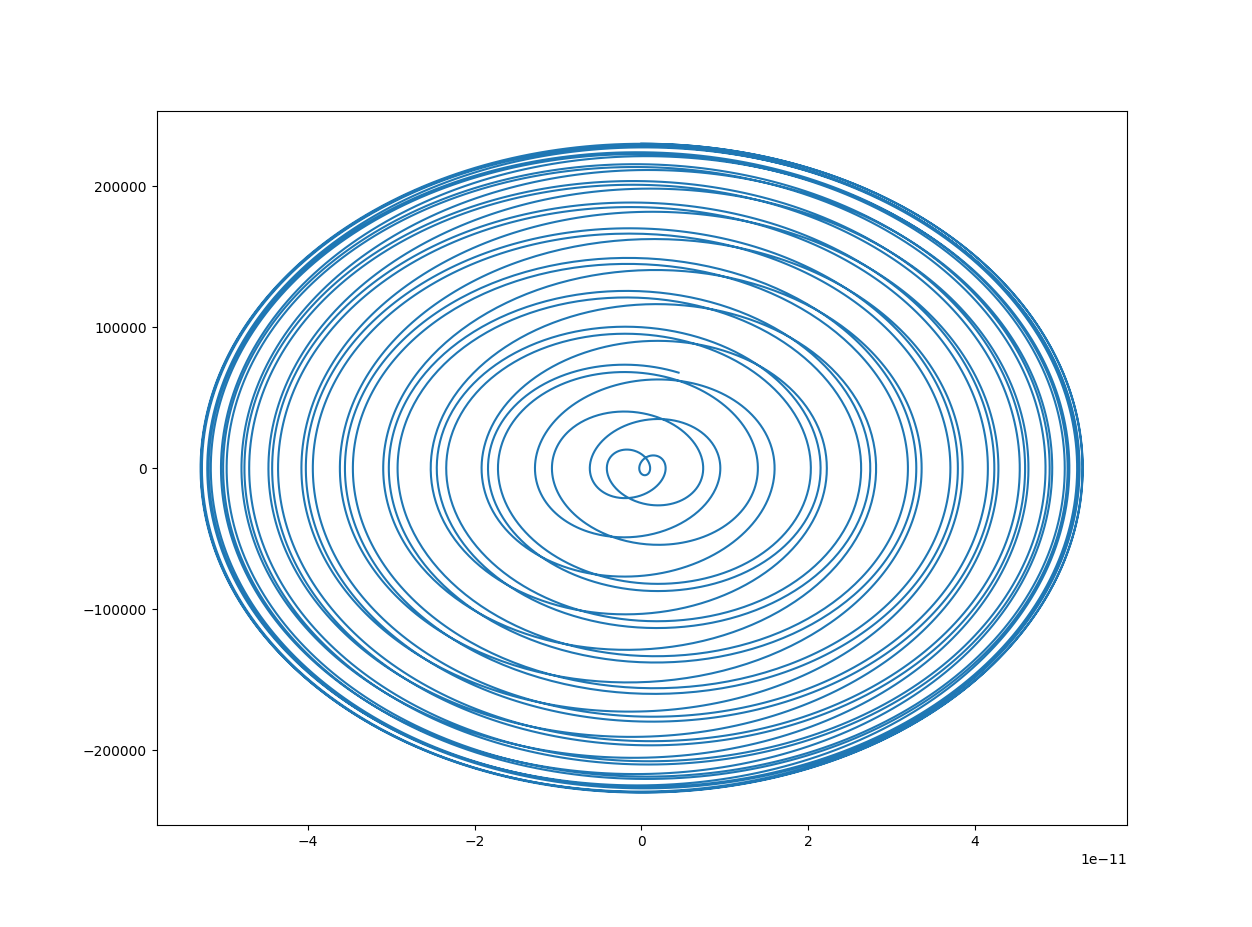
\includegraphics[width=14cm]{TP/Images/ED2_Zeeman2.png}    
\end{center}
%-------------------------------------------------------------------------------
\end{Answer}
%-------------------------------------------------------------------------------
%-------------------------------------------------------------------------------
\subsection{Ceintures de Van Halen}
%-------------------------------------------------------------------------------
%-------------------------------------------------------------------------------
Les ceintures de Van Halen sont des régions autour de la terre dans lesquelles les particules chargées issues du soleil peuvent se retrouver piégées. Le champ magnétique terrestre dévie les particules de leur trajectoire vers la terre en leur faisant suivre les lignes de champ. Nous allons observer les trajectoire des protons dans la première ceinture située approximativement à une distance de 2 rayons terrestres du centre de la terre. On donne les valeurs 
\begin{lstlisting}
q0 = 1.6e-19  # C, charge du proton
m0 = 1.67e-27 # kg, masse du proton
\end{lstlisting}

Le champ magnétique terrestre peut être approché par un dipôle magnétique  : il est représenté par son origine $O$, au centre de la terre, par son moment magnétique $\vec \mu$ dont la direction est proche de l'axe de la terre. La valeur numérique estimée est $\|\vec \mu\| = 7,7.10^{22}\text{A}\cdot \text{s}^{-2}$.

Les vecteurs dans {\sc Python} seront représentés par un tableau {\sc numpy} avec la troisième coordonnée indiquant l'axe de la terre
\begin{lstlisting}
mu = np.array([0.0, 0.0, 7.7e22])
\end{lstlisting}

Le champ magnétique en un point $M$ est alors, en notant $r = \left\|\overrightarrow{OM}\right\|$ et $\displaystyle \vec u = \frac 1 r\overrightarrow{OM}$,
\[\overrightarrow{B(M)} = \frac{\mu_0}{4\pi}\frac{3(\vec \mu.\vec u)\vec u - \vec \mu}{r^3}\]
On a $\mu_0=4\pi10^{-7}\text{kg}\cdot\text{m}\cdot\text{A}^{-2}\cdot\text{s}^{-2}$ et on notera \type{mu0} la valeur de $\displaystyle \frac{\mu_0}{4\pi}$ : \type{mu0 = 1.0 e-7}.

Le produit scalaire de deux vecteurs représentés par des tableaux \type{u} et \type{v} de même taille se calcule par \type{np.dot(u, v)}, leur produit vectoriel par \type{np.cross(u, v)}

%-------------------------------------------------------------------------------
%-------------------------------------------------------------------------------
\begin{Exercise}\it
Écrire une fonction \type{B(M)} qui calcule le champ magnétique en un point $m$ représenté par un tableau {\sc numpy} de taille 3 (il représente aussi le vecteur $\overrightarrow{OM}$). 
\end{Exercise}
%--------------------------------------------------------------------------
\begin{Answer}
\begin{lstlisting}
def B(M):
    r = np.dot(M, M)**0.5 
    u = (1/r)*M
    return mu0*(3*np.dot(mu,u)*u -mu)/(r**3)
\end{lstlisting}
\end{Answer}
%--------------------------------------------------------------------------
%--------------------------------------------------------------------------
L'équation différentielle dont on cherche les solution est alors
\[m\frac{\overrightarrow{\d^2 M}}{\d t^2} = q\frac{\overrightarrow{\d M}}{\d t}\wedge \overrightarrow{B(M)}\]
Cette équation va se traduire en un système différentiel à 6 variables : les 3 coordonnées de $x$, $y$ et $z$, coordonnées de $M$, et les coordonnées du vecteur vitesse. 
%-------------------------------------------------------------------------------
%-------------------------------------------------------------------------------
\begin{Exercise}\it
Écrire une fonction \type{phi(u, t)} qui décrit le système différentiel, elle reçoit deux variables, un tableau de taille 6 et un flottant pour le temps (qui n'intervient pas) et doit renvoyer un tableau de taille 6.  
\end{Exercise}
%--------------------------------------------------------------------------
\begin{Answer}
\begin{lstlisting}
def phi(u, t):
    M = u[0:3]
    V = u[3:6]
    dM = np.zeros(6)
    dM[0:3] = V
    dM[3:6] = q0*np.cross(V, B(M))/m0
    return dM
\end{lstlisting}
\end{Answer}
%-------------------------------------------------------------------------------
%-------------------------------------------------------------------------------
Les unités de base pour les conditions initiales sont le rayon de la terre pour la position initiale et une fraction de la vitesse de la lumière pour la vitesse initiale. Par exemple :
\begin{lstlisting}
RT = 6.4e6
c = 3.0e8
u0 = np.array([0, 2*RT, 0, 0, 0.25*c, 0.1*c])
\end{lstlisting}
%-------------------------------------------------------------------------------
%-------------------------------------------------------------------------------
\begin{Exercise}\it
Tracer la courbe intégrale d'une solution sur $[0; 5]$.
\end{Exercise}
%--------------------------------------------------------------------------
\begin{Answer}
\begin{lstlisting}
T = np.linspace(0, 5, 10000)
u0 = np.array([0, 2*RT, 0, 0, 0.25*c, 0.1*c])
U= odeint(phi, u0, T)
X = U[ : , 0]
Y = U[ : , 1]
Z = U[ : , 2]
fig=plt.figure()
ax=Axes3D(fig, auto_add_to_figure = False)
fig.add_axes(ax)
ax.plot(X, Y, Z)
plt.show()
\end{lstlisting}
%--------------------------------------------------------------------------
\begin{center}
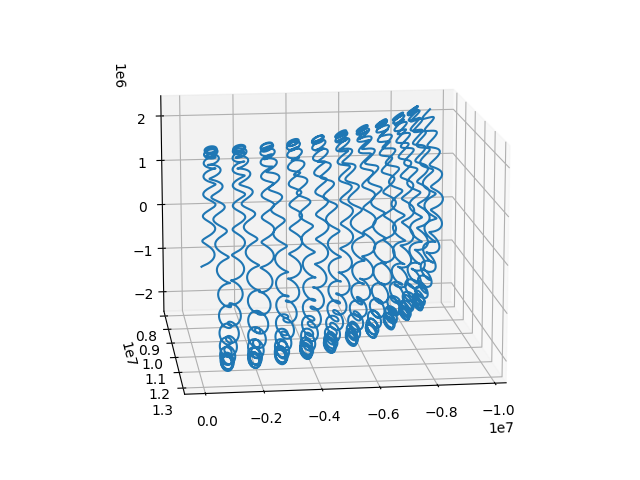
\includegraphics[width=14cm]{Cours/Images/ED2_vanHalen1.png}    
\end{center}
%--------------------------------------------------------------------------
\begin{center}
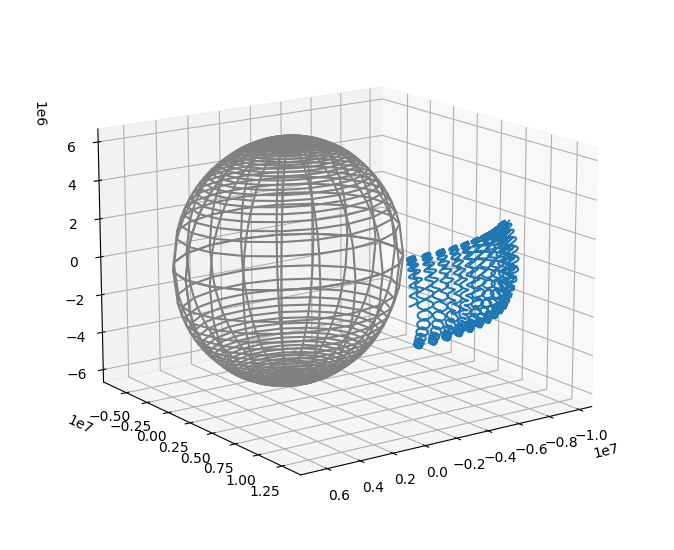
\includegraphics[width=14cm]{Cours/Images/ED2_vanHalen2.png}    
\end{center}
%--------------------------------------------------------------------------
\end{Answer}
%--------------------------------------------------------------------------
%--------------------------------------------------------------------------
On peut souhaiter représenter la terre pour voir la position relative de la trajectoire.
\begin{lstlisting}
r = np.linspace(0, RT, 30)
phi = np.linspace(0, 2*np.pi, 20)
R, Phi = np.meshgrid(r, phi)
X1 = R*np.cos(Phi)
Y1 = R*np.sin(Phi)
Z1 = (RT**2 - R**2)**0.5
ax.plot_wireframe(X1, Y1, Z1, color = "gray")
ax.plot_wireframe(X1, Y1, -Z1, color = "gray")
ax.set_xlim([-d*1.1, d*1.1])
ax.set_ylim([-d*1.1, d*1.1])
ax.set_zlim([-1.2*RT, 1.2*RT])
plt.show()
\end{lstlisting}
\type{meshgrid} construit deux tableaux à deux dimension à partir de deux tableaux à une dimension en répétant les valeurs sur les colonnes pour le premier tableau et sur les lignes pour le second.
\begin{lstlisting}
>>> np.meshgrid([1, 2, 3], [4, 5, 6, 7])
[array([[1, 2, 3],
       [1, 2, 3],
       [1, 2, 3],
       [1, 2, 3]]), 
array([[4, 4, 4],
       [5, 5, 5],
       [6, 6, 6],
       [7, 7, 7]])]
\end{lstlisting}

